\batchmode
\makeatletter
\def\input@path{{/home/moritz/Home/Projekte/Minetest/minetest/mods/advtrains/assets/}}
\makeatother
\documentclass[english]{paper}
\usepackage[T1]{fontenc}
\usepackage[latin9]{inputenc}
\usepackage{geometry}
\geometry{verbose,tmargin=1cm,bmargin=1cm,lmargin=1cm,rmargin=1cm}
\setlength{\parindent}{0bp}
\usepackage{graphicx}
\usepackage{babel}
\begin{document}

\title{Minetest Mod - Advanced Trains {[}advtrains{]}}

\title{Interlocking System Guide}
\maketitle

\section{Introduction}

In real-world railways, a so-called interlocking system is a set of
railway signals and trackside equipment. Its purpose is to prevent
conflicting train movements which otherwise could result in derailing
or colliding trains. If you want more information, just search for
``railway interlocking'' on the internet.

Real-world interlocking systems perform this task by setting routes.
A route is a path along a track that a train can safely pass. To set
a route for a train, the signalman (the operator of a signal box)
has to set switches (turnouts) to the correct position and lock them
in order to make a signal for a train show ``Proceed''. In newer
systems, this is done automatically by the interlocking system. A
route can not be set if switches are locked to a wrong position by
another route or if any portion of the route is occupied by a train.

The interlocking system in this Minetest mod tries to follow real-world
interlocking systems as far as applicable. It divides tracks into
track sections and implements a route setting mechanism following
the same principle.

However, for the sake of simplicity of implementation and usage, not
all concepts of real-world interlocking have been taken over. Especially,
there is no mechanism for overlap.

If you are looking for a place to learn how real-world interlocking
systems work, have a look at ``SimSig''. By looking at their simulations,
you can obtain experience on how to set up your own interlocking systems
in AdvTrains. The SimSig glossary is a good place to look up unknown
terms in this document.

\section{Setting up track sections}

In the real world, a line of track is divided into so-called track
sections, or track circuits. Those systems often can not tell where
exactly a train is, but only which track sections it occupies. A route
can never be set through an occupied track section.

A track section often covers:
\begin{itemize}
\item A section on a main running line, between two signals
\item A single turnout
\item A rail crossing, or a set of turnouts acting as a double/single slip
switch
\item A siding
\end{itemize}
You will find some examples on how to interlock certain patterns later.

\subsection{Track Circuit Breaks}

In this mod, you will not directly configure the locations of track
sections. Instead, you designate the borders of each track section
using a special node, the Track Circuit Break, abbreviated TCB.

For example, if you want to create a track section for a piece of
a main running line, you set up two TCBs at the ends of this track
circuit.

Setting up a TCB works as follows:
\begin{enumerate}
\item Place a TCB node somewhere near the place where the circuit break
is going to be located.
\item Right-click the TCB node
\item Punch the rail which should act as TCB
\end{enumerate}
The result should look like this:

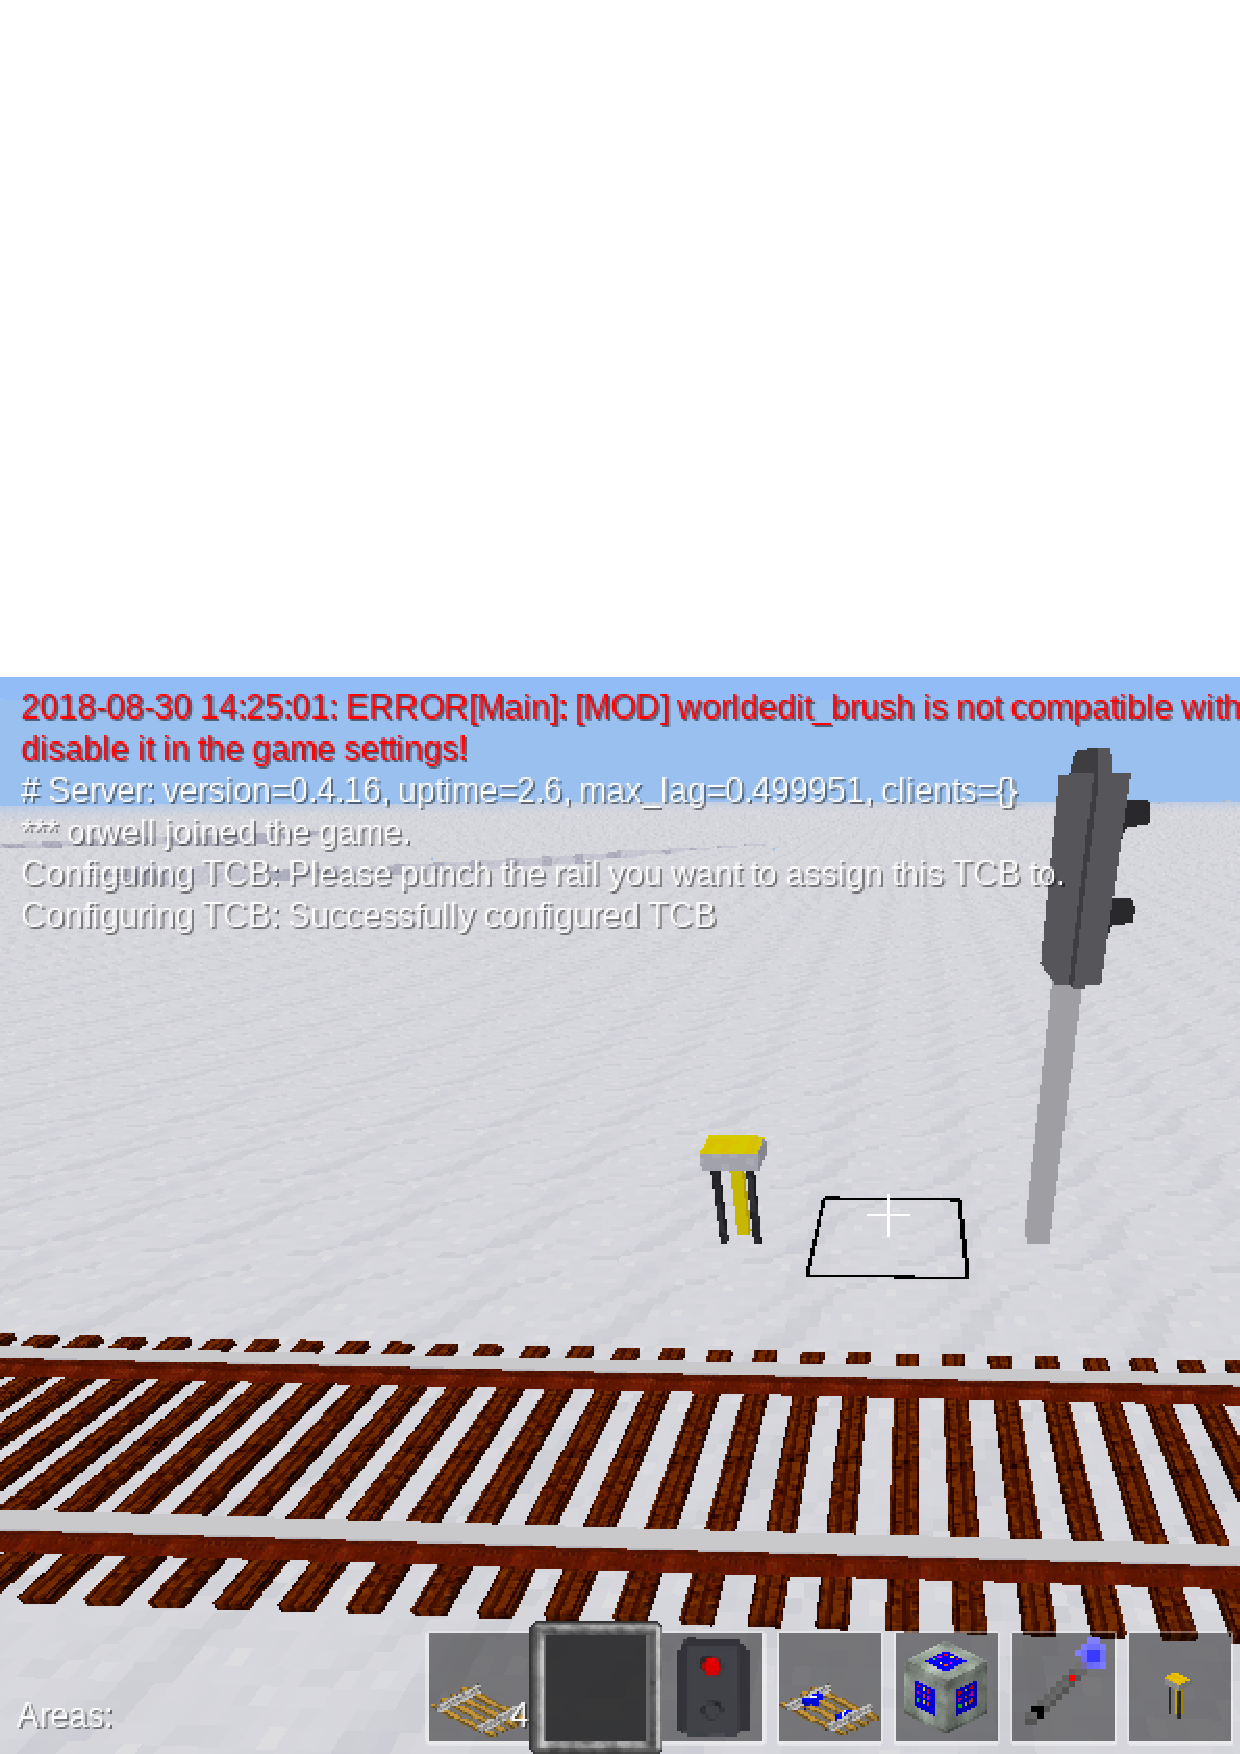
\includegraphics[width=10cm]{0_home_moritz_Home_Projekte_Minetest_minetest_m___s_assets_lyx_img_screenshot_20180830_142551.png}

Now you have assigned the TCB node to a rail. Right-click the TCB
node once again. This will bring up a form which looks as follows:

\includegraphics[width=10cm]{1_home_moritz_Home_Projekte_Minetest_minetest_m____lyx_img_Bildschirmfoto_2018-08-30_14-26-35.png}

You see that the form is divided in side A and side B. To designate
where each side is, a marker is displayed on the rail. You can always
make this marker show up by punching the TCB node, and remove it by
punching the marker. Both sides are shown as ``End of interlocking''.
This means that there is no track section set up at this place.

You should repeat this procedure once again a few meters away from
the first TCB to create a second TCB on the same track.

\includegraphics[width=10cm]{2_home_moritz_Home_Projekte_Minetest_minetest_m____lyx_img_Bildschirmfoto_2018-08-30_14-32-48.png}

Once you have both bordering TCBs set up, you can now create the actual
track section. To do this:
\begin{enumerate}
\item Right-click one of the TCBs
\item Locate the correct side (A or B) to create the track section
\item Click ``Create interlocked Track Section'' in the formspec on the
chosen side.
\end{enumerate}
Now, the text on the formspec has changed. It shows something like
this:

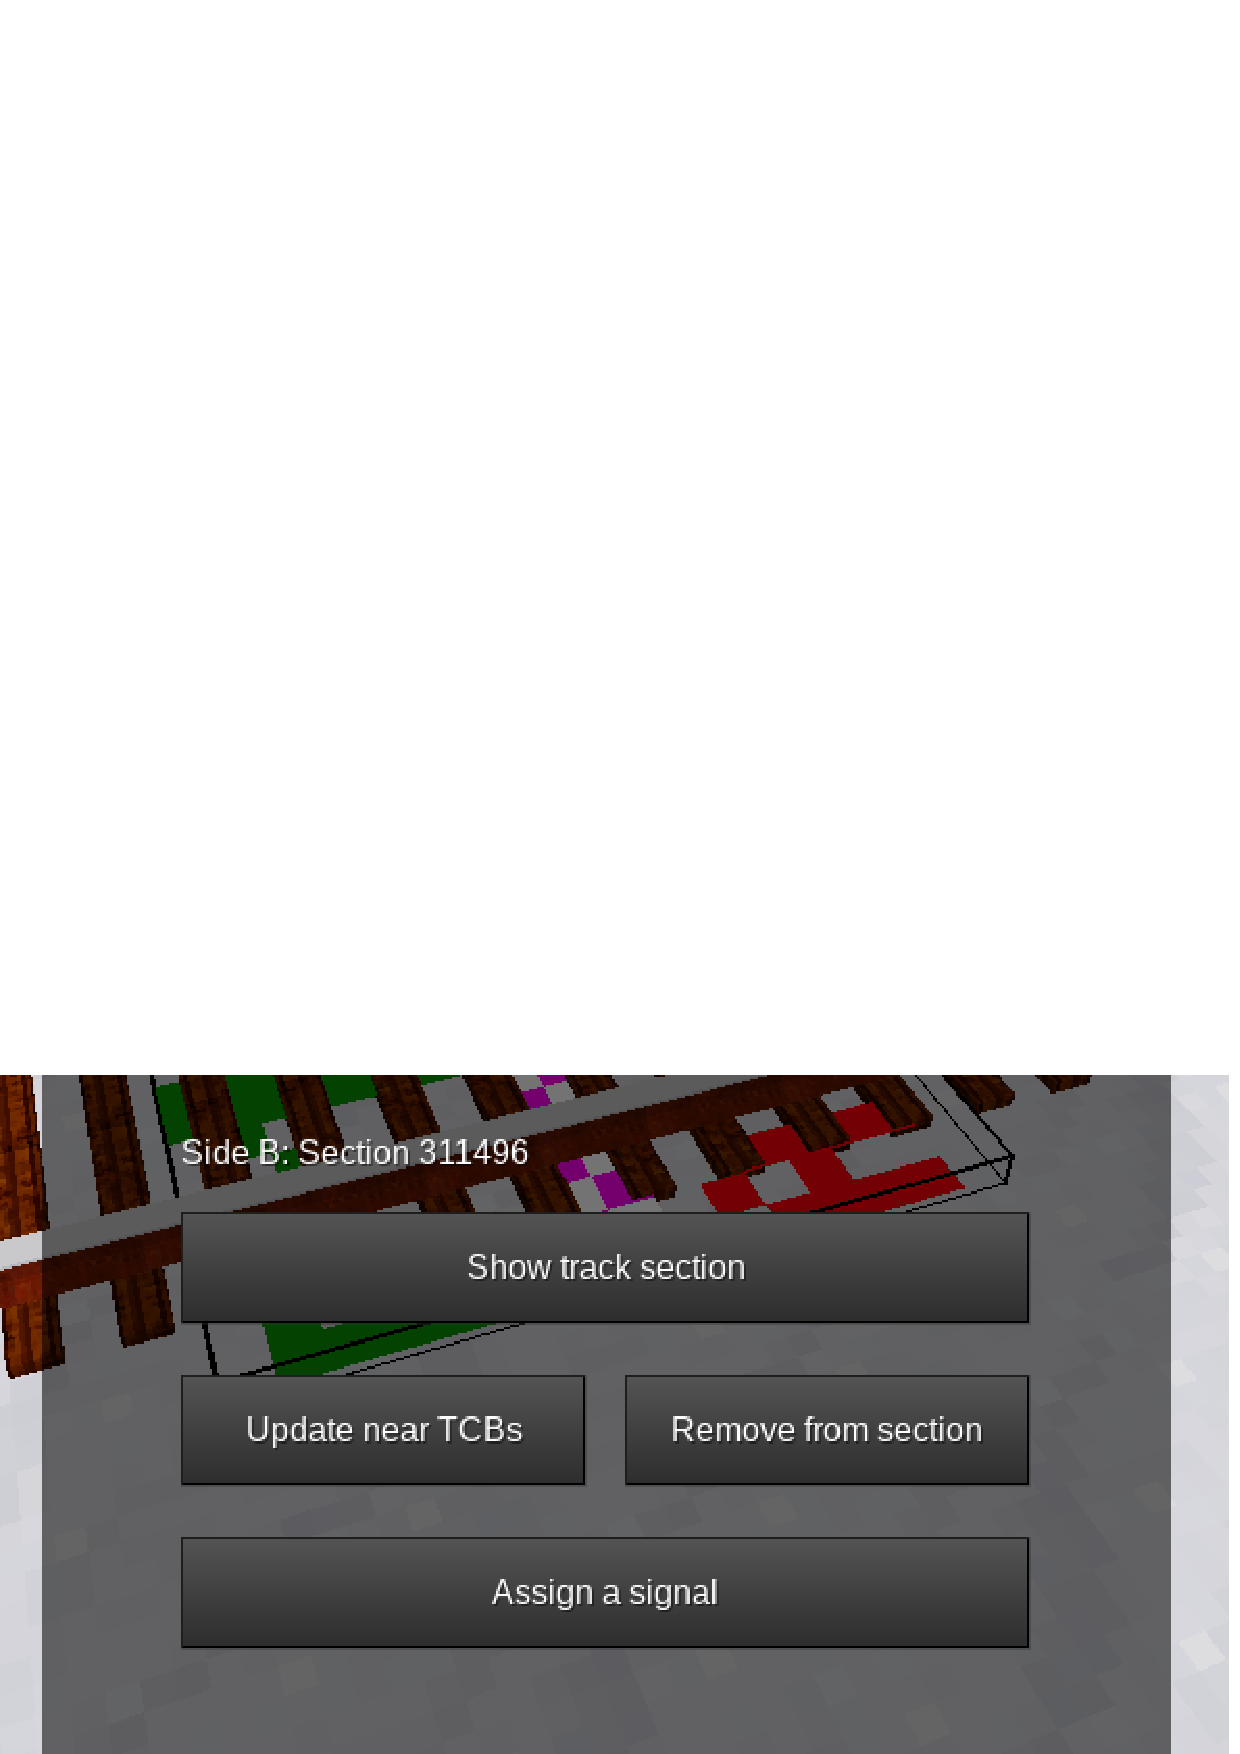
\includegraphics[width=5cm]{3_home_moritz_Home_Projekte_Minetest_minetest_m____lyx_img_Bildschirmfoto_2018-08-30_14-27-25.png}

Clicking ``Show Track Section'' brings up another formspec:

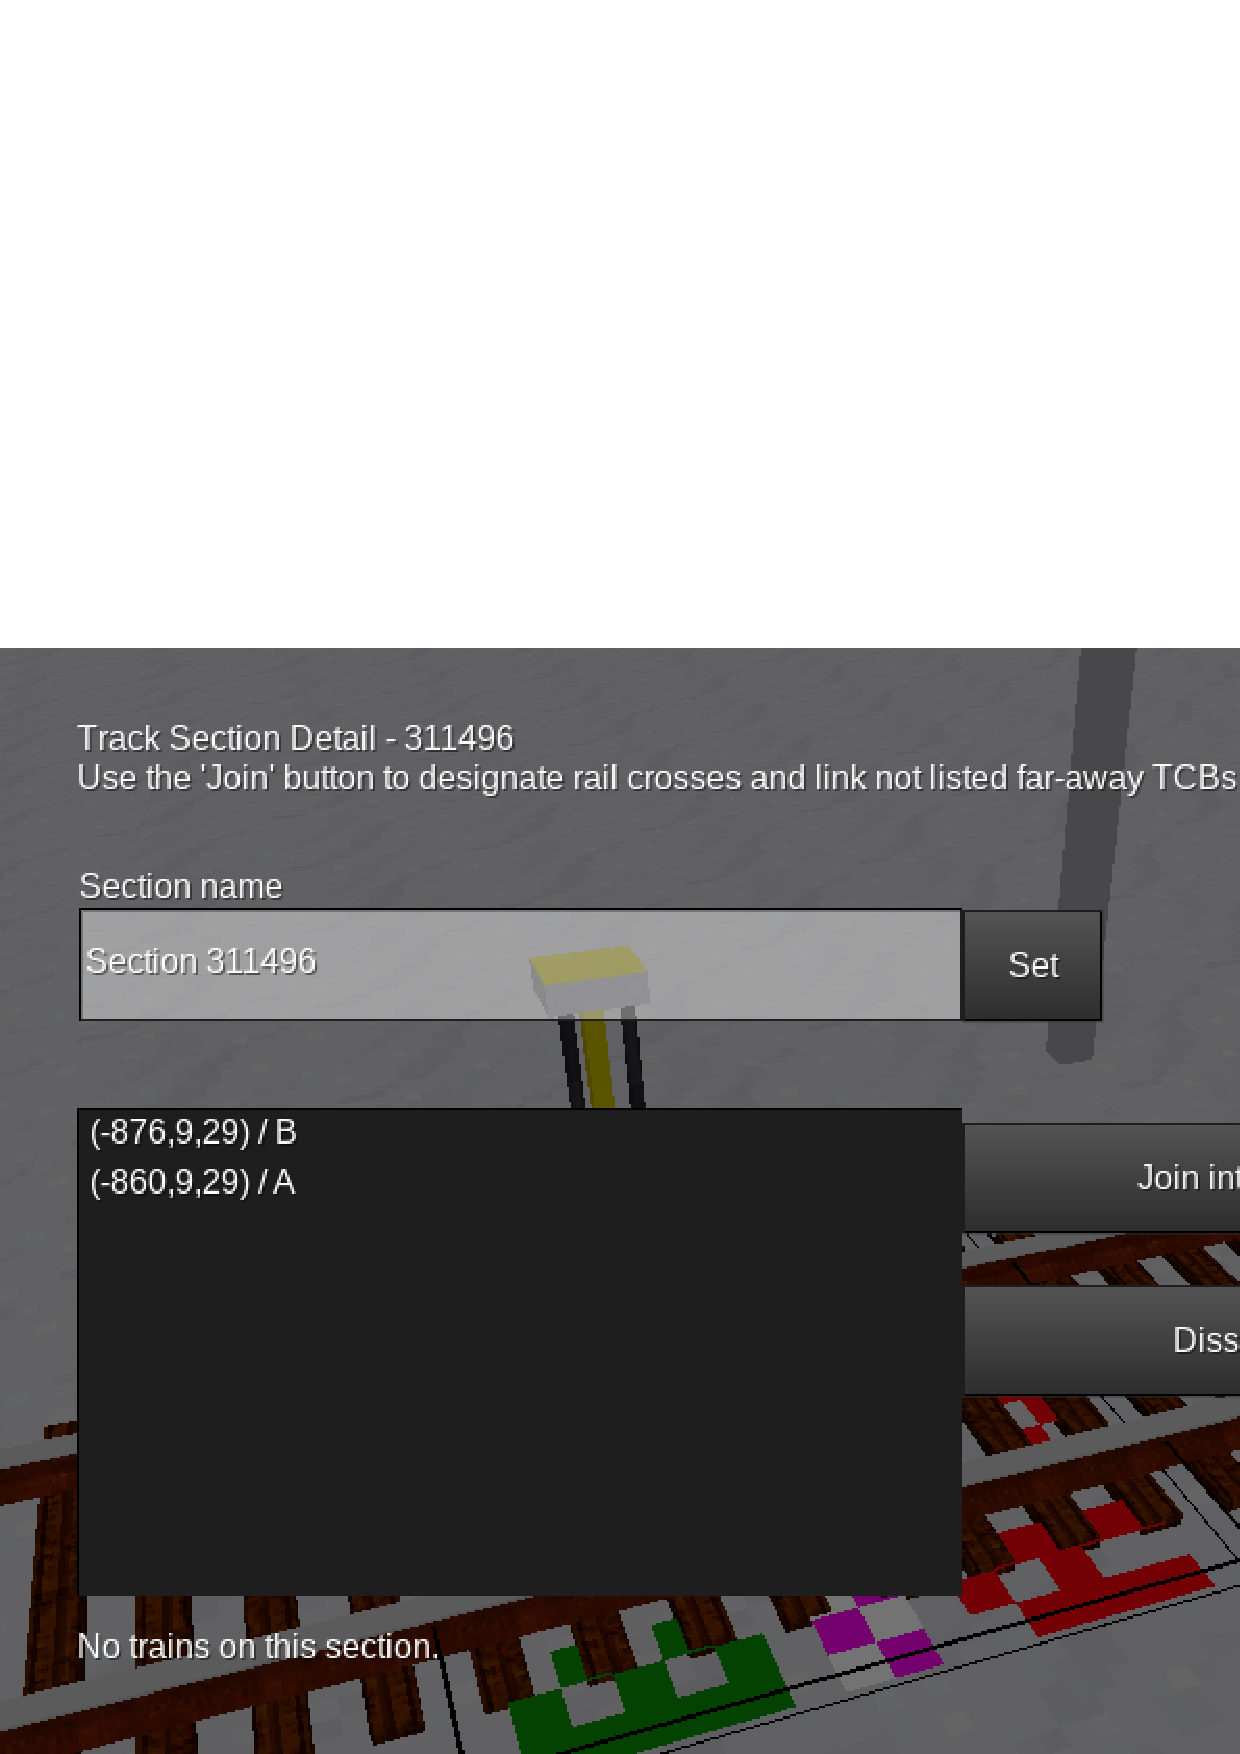
\includegraphics[width=5cm]{4_home_moritz_Home_Projekte_Minetest_minetest_m____lyx_img_Bildschirmfoto_2018-08-30_14-28-32.png}

On the top, you see a list of all TCBs that border this track section.
In your case, there should be two TCBs listed. If there's only one,
head over to \ref{subsec:Long-track-sections,}. You should now select
a name for the track section, to identify it later.

The same procedure is applicable when you create a turnout track section,
except that you have to set up three or more TCBs.

The AdvTrains interlocking system allows you to add more TCBs after
you have created a track section. This works without problems in most
cases. For example, you can easily insert a turnout into an already
set-up track section and create another TCB behind it, and AdvTrains
will automatically detect the existing track section. Problems arise
only if you try to insert a TCB in-between a section, in which case
both sides of the TCB will end up assigned to the same section. The
code currently does not handle this case properly, so try to avoid
this situation by all means. As a last resort, you can always dissolve
a faulty track section, as described in the next chapter.

\subsection{Long track sections, crossings and other edge cases\label{subsec:Long-track-sections,}}

\subsubsection{Very long track sections}

If you try to set up a track section that is longer than 1000 nodes,
advtrains won't recognize the TCB at the other end because of a safety
limit in the traverser function, which is supposed to prevent deadlocks.
This case has happened when the Track Section overview screen only
shows one TCB in the list. The procedure for this is as follows:
\begin{enumerate}
\item Go to the second TCB (the one that wasn't recognized). It should show
``End of Interlocking'' on the relevant side.
\item Click ``Create interlocked track section''. The section created
will be different from the one that is already present.
\item In the track section overview, click ``Join into other section''
\item Go back to the first TCB, bring up the Track Section overview screen
of the first track section and click ``Join with ???''
\end{enumerate}
The other, missing TCB should now appear in the list. If you accidentally
started such a joining procedure, click the ``X'' button on the
right.

\subsubsection{Rail crosses}

Since rail crosses are created by laying tracks across each other
without logical connection, there's no way for advtrains to know whether
rails cross each other.

Rail crossings in interlocking systems are always one single track
section, which in most cases has 4 TCBs adjacent.

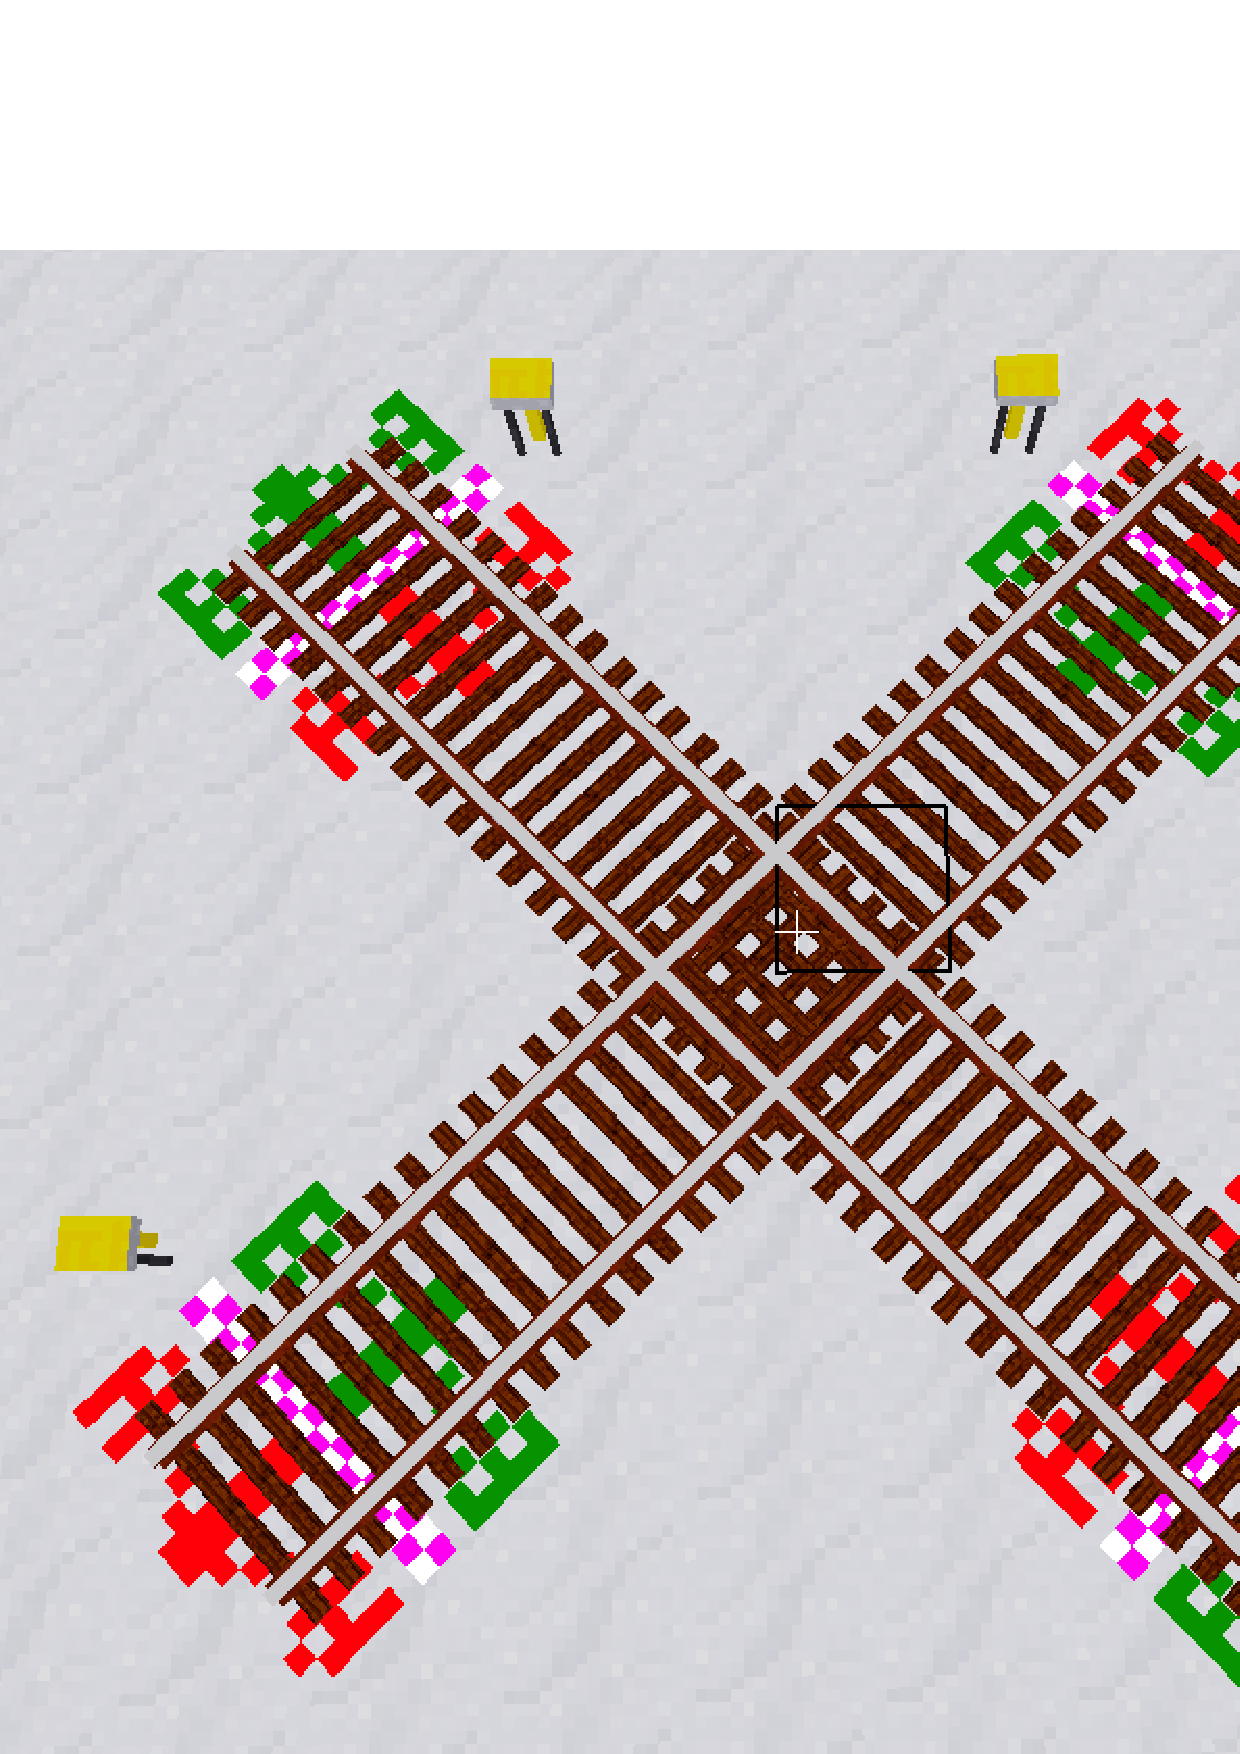
\includegraphics[width=5cm]{5_home_moritz_Home_Projekte_Minetest_minetest_m____lyx_img_Bildschirmfoto_2018-08-30_14-51-25.png}

The procedure is quite similar to the one for long sections: First,
create two track sections for the branches, and then use the ``Join''
function to merge both sections into one.

\subsubsection{Deleting and re-adding single TCBs to a section}

In some occasions, for example when you remove a siding or a crossover,
it can be necessary to unassign a TCB from a track section. There
are multiple ways to do this:
\begin{itemize}
\item In the TCB form, click the ``Remove from section'' button
\item In the track section form, first select the TCB in the list and then
click ``Unlink selected TCB''
\end{itemize}
The result is that the TCB shows ``End of Interlocking'' and the
section does not list the TCB as an endpoint anymore.

The other case is adding a siding or a crossover, in which case one
or more TCBs still show ``End of Interlocking'' although they should
be part of a section:
\begin{itemize}
\item Go to another TCB that is registered in the track section and click
``Update near TCBs''
\item If that did not work, follow the procedure of creating a long track
section
\end{itemize}

\subsubsection{Dissolving sections}

If you made a mistake setting up something and you don't see any other
way to fix a misconfigured track section, you can always delete it
using the ``Dissolve section'' button. This operation removes the
track section and sets all TCBs that previously belonged to the section
as ``End of Interlocking''. This will always work and lets you start
over new with setting up track sections.

\subsection{Interlocking patterns}

This section is supposed to show some examples on how you should set
up track sections on certain track configurations.

\section{Signals and routes}

Signals are appliances that can give instructions to trains. That
can be the permission to proceed, a speed restriction, or other information.

There are 2 types of signals:
\begin{itemize}
\item Static signals always display the same information to the train. This
can be a speed restriction (or the end of one), a disallowal to proceed
as shunt move or similar things. In most cases, these are signs.
\item Variable signals are what most people would call a ``signal''. Its
function is to inform trains about whether and at which speed they
can proceed into the next section safely.
\end{itemize}

\subsection{Signal Influence Point}

Every signal is associated to a track on which the instruction should
be followed. Signals are usually placed right next to the track on
the right side. Human observers do know then that the signal belongs
to the track left of it, however, train safety systems (like the one
in advtrains) can not.

This is the reason why a so-called ``influence point'' needs to
be assigned to any signal that should actually give instructions to
trains, should the driver (if even there is one) fail to recognize
the instructions.

Depending on the signal and the mod that adds the signal, there are
different ways to configure this. Signals integrated into advtrains
behave as follows:
\begin{itemize}
\item Static signals and all red-green light signals from core advtrains
that are not assigned to a TCB can be configured by holding the ``Sneak''
key and then right-clicking the signal
\item All signals that are assigned to a TCB can be configured by first
right-clicking them, then selecting ``Influence Point'' in the signalling
formspec.
\end{itemize}
The small formspec that opens allows you to set and later view or
clear the Influence Point. To set the influence point, click the ``Set''
button, face towards the signal and punch a rail about 2m in front
of the signal. A small marker will be shown, indicating success. To
cancel setting an influence point, punch anything other. (note that
then the influence point remains unset, regardless of its previous
state)

The advtrains-internal train safety system ensures that the train
always obeys any restrictions imposed by signals, if (and only if)
the influence point is set properly.

\subsection{Main and Shunt signals}

While static signals are mainly used for speed restrictions, the interesting
ones are variable signals. Of course, you can always control any variable
signal by traditional means (mesecons, digiline, right-click) if the
signal allows it, but that misses the point of this interlocking system.

In the following sections, we will talk about main signals. By this,
we mean a variable signal that can display both a ``Danger'' aspect
(trains are not allowed to proceed) and at least one ``Proceed''
aspect (train may proceed as train/shunt move, with optional speed
restriction), which act as an ``entry signal'' for one or multiple
routes.

\subsection{The concept of routes}

A so-called route is a locked path between two main signals, which
locks all turnouts in the correct position. Its purpose is to offer
a train a path on which it can safely proceed without interfering
with any other train. A route always incorporates and locks one to
multiple track sections, starting with the one that lies directly
behind the ``entry'' signal.

Example: Imagine a station with 2 platforms on a single track running
line. We are looking at signal A. You probably want trains coming
from the right to go into platform 1 or into platform 2, so you need
to program 2 routes.

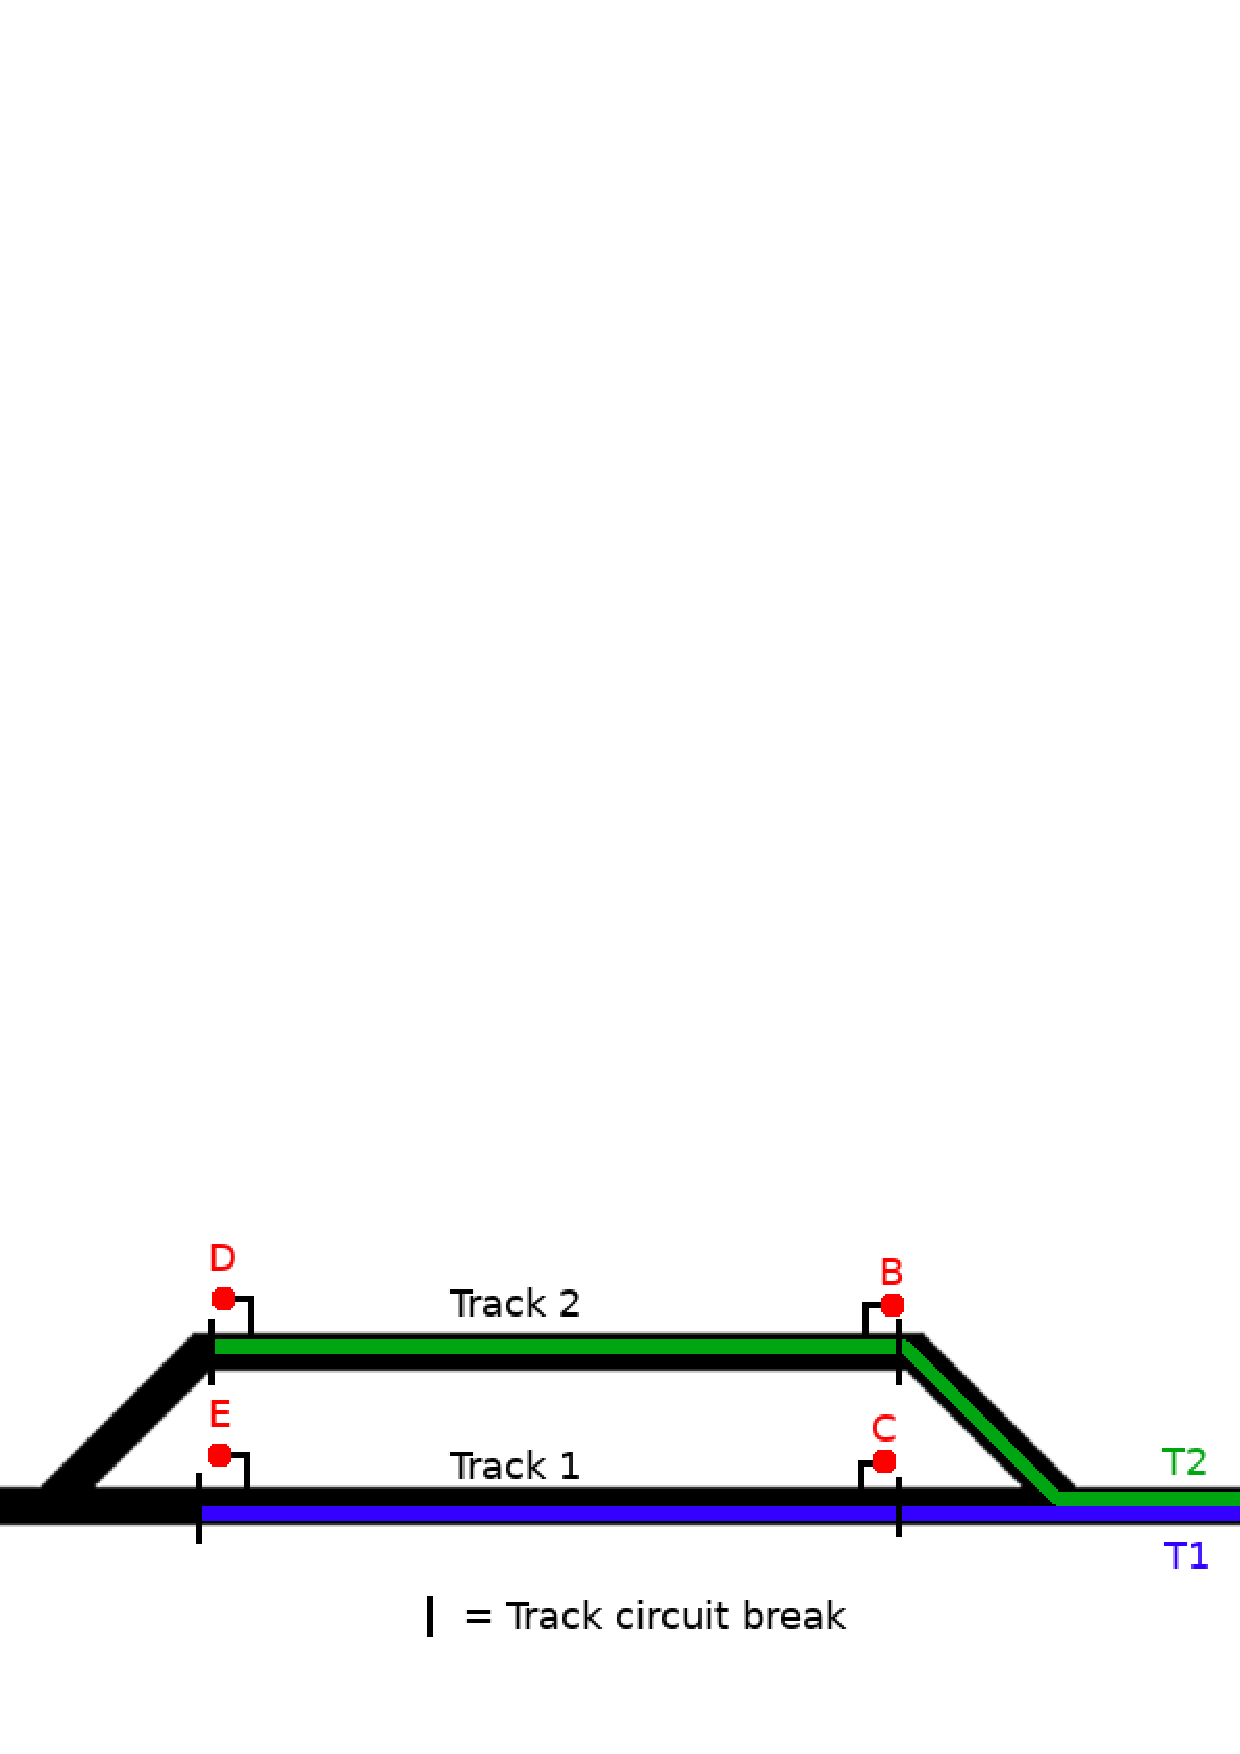
\includegraphics[width=7cm]{6_home_moritz_Home_Projekte_Minetest_minetest_mods_advtrains_assets_lyx_img_route_ex1.png}

This leads us to the most important aspect of route programming: Routes
always start at a signal (A) and end at a signal facing in the \textbf{same
direction} (D and E), not at an opposite-facing signal (B and C).
There are only few exceptions, we'll cover this later.

When you set a route to make a train proceed on it, the interlocking
system ensures that:
\begin{itemize}
\item There are no rail vehicles on the route
\item All turnouts are set to the correct position and it is impossible
to move them
\item No other routes can be set that would in any way conflict with this
route
\end{itemize}
For this to work, you need to specify all track sections the train
will pass along, as well as the positions of all turnouts that need
to be locked. Those are not only the turnouts that lay directly on
the train's route, but also some turnouts on adjacent tracks, the
so-called flank protection.

The purpose of flank protection is to prevent runaway trains and/or
wagons to pass into a route. This is achieved by setting nearby turnouts
to a position that points ``away'' from the route. Example:

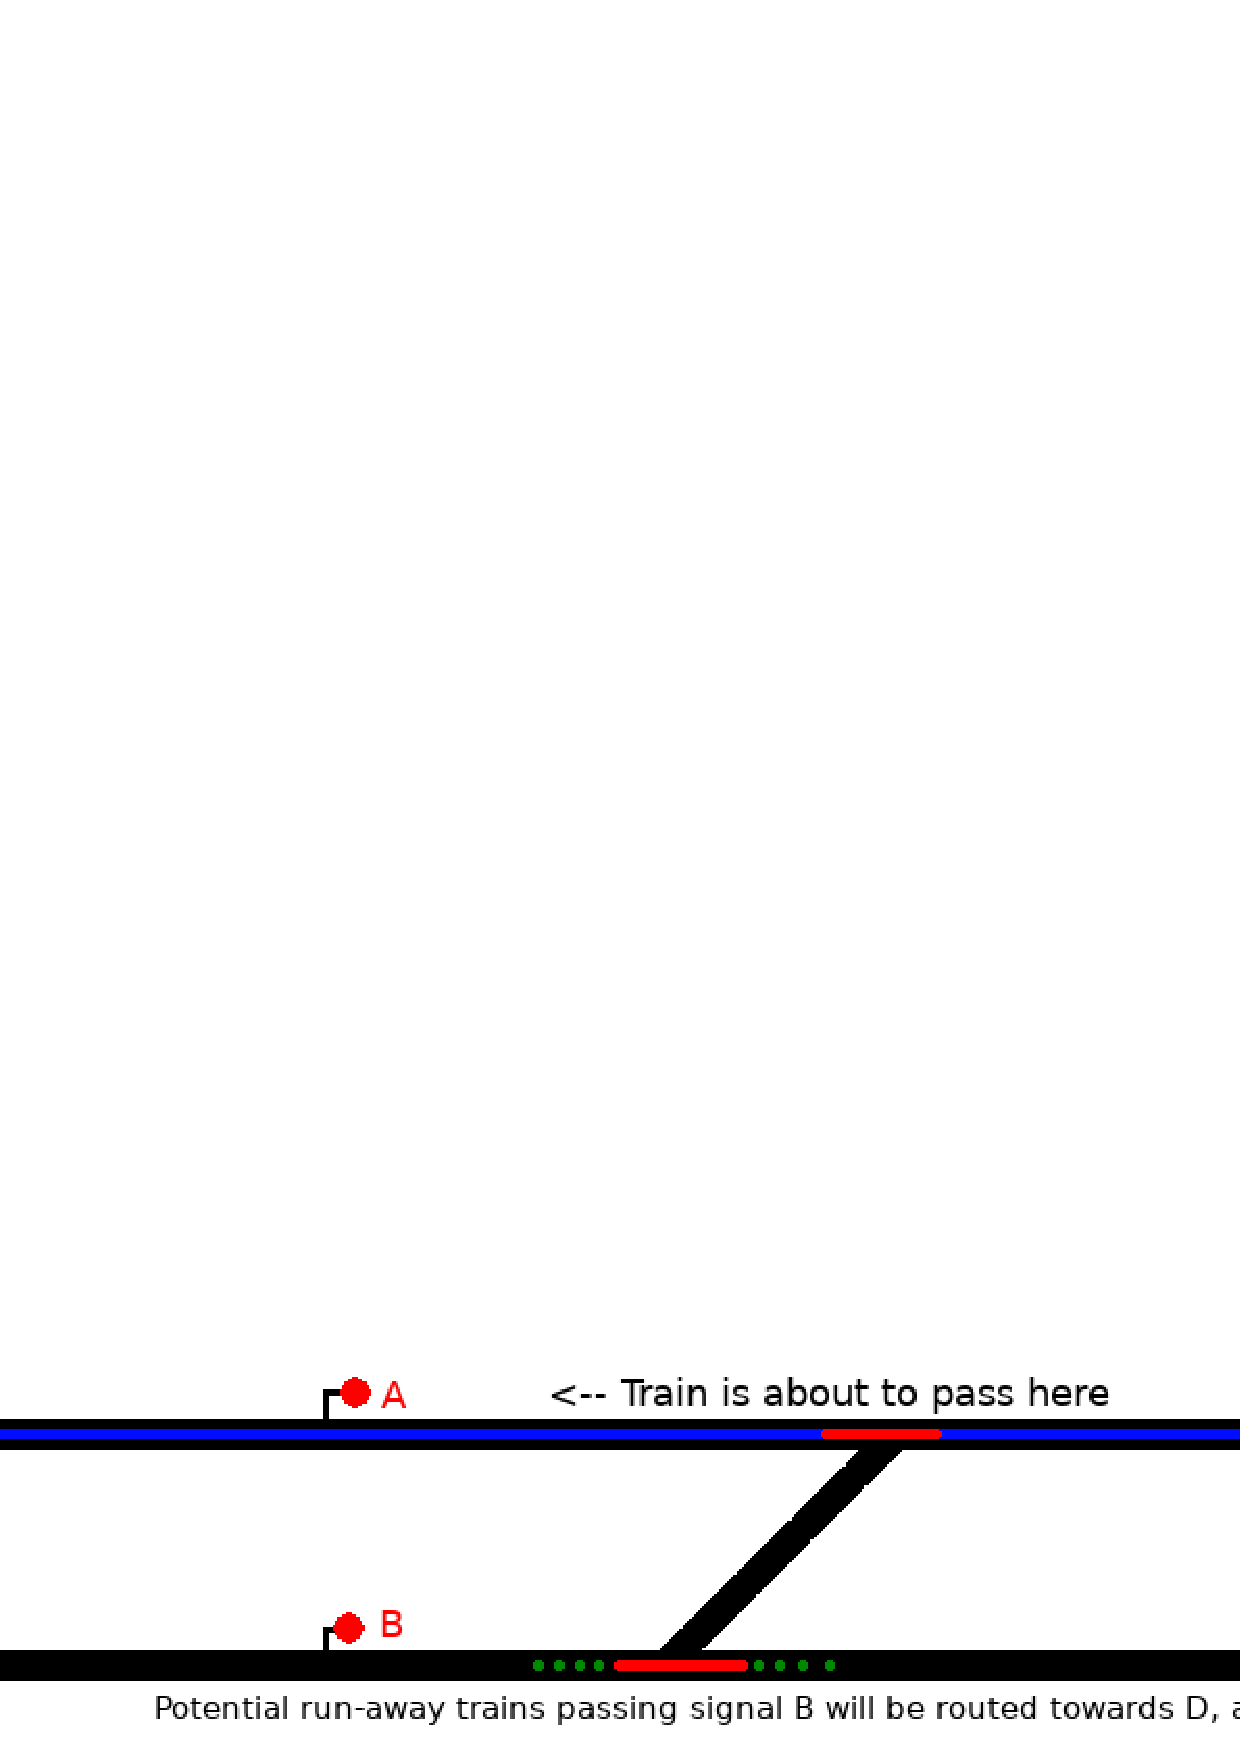
\includegraphics[width=7cm]{7_home_moritz_Home_Projekte_Minetest_minetest_mods_advtrains_assets_lyx_img_route_ex2.png}

The upper turnout, of course, needs to be locked in straight (normal)
position, while the lower one is not relevant for the route itself.
But what if the lower turnout was set to the diverging (reverse) position
and the driver of another train approaching signal B fails to see
the red light? This train would crash into the first one. To minimise
danger, that other train would need to be routed towards signal D.

There are, of course, situations, where both positions of a turnout
would conflict with a route equally. In those situations, there's
nothing you can do and no flank lock needs to be set.

\subsection{Assigning main signals to TCBs}

Main signals in the advtrains interlocking system are positioned -
like in real life - at the border of track sections, because routes
also start and end there. For advtrains to know from which signal
which routes can be set, you need to assign the signal to a TCB.

To do this, perform the following steps:
\begin{enumerate}
\item If not already happened, set up a TCB (you don't need to, but are
advised to, configure track sections there)
\item Place the signal a few meters in front of the TCB, so that trains
stopping at the signal do never pass the TCB
\item Locate the side of the TCB which points in the direction that trains
will proceed past the signal, as shown in the figure below.
\item Right-click the TCB, and click ``Assign a signal'' on this side.
\item Punch the signal.
\end{enumerate}
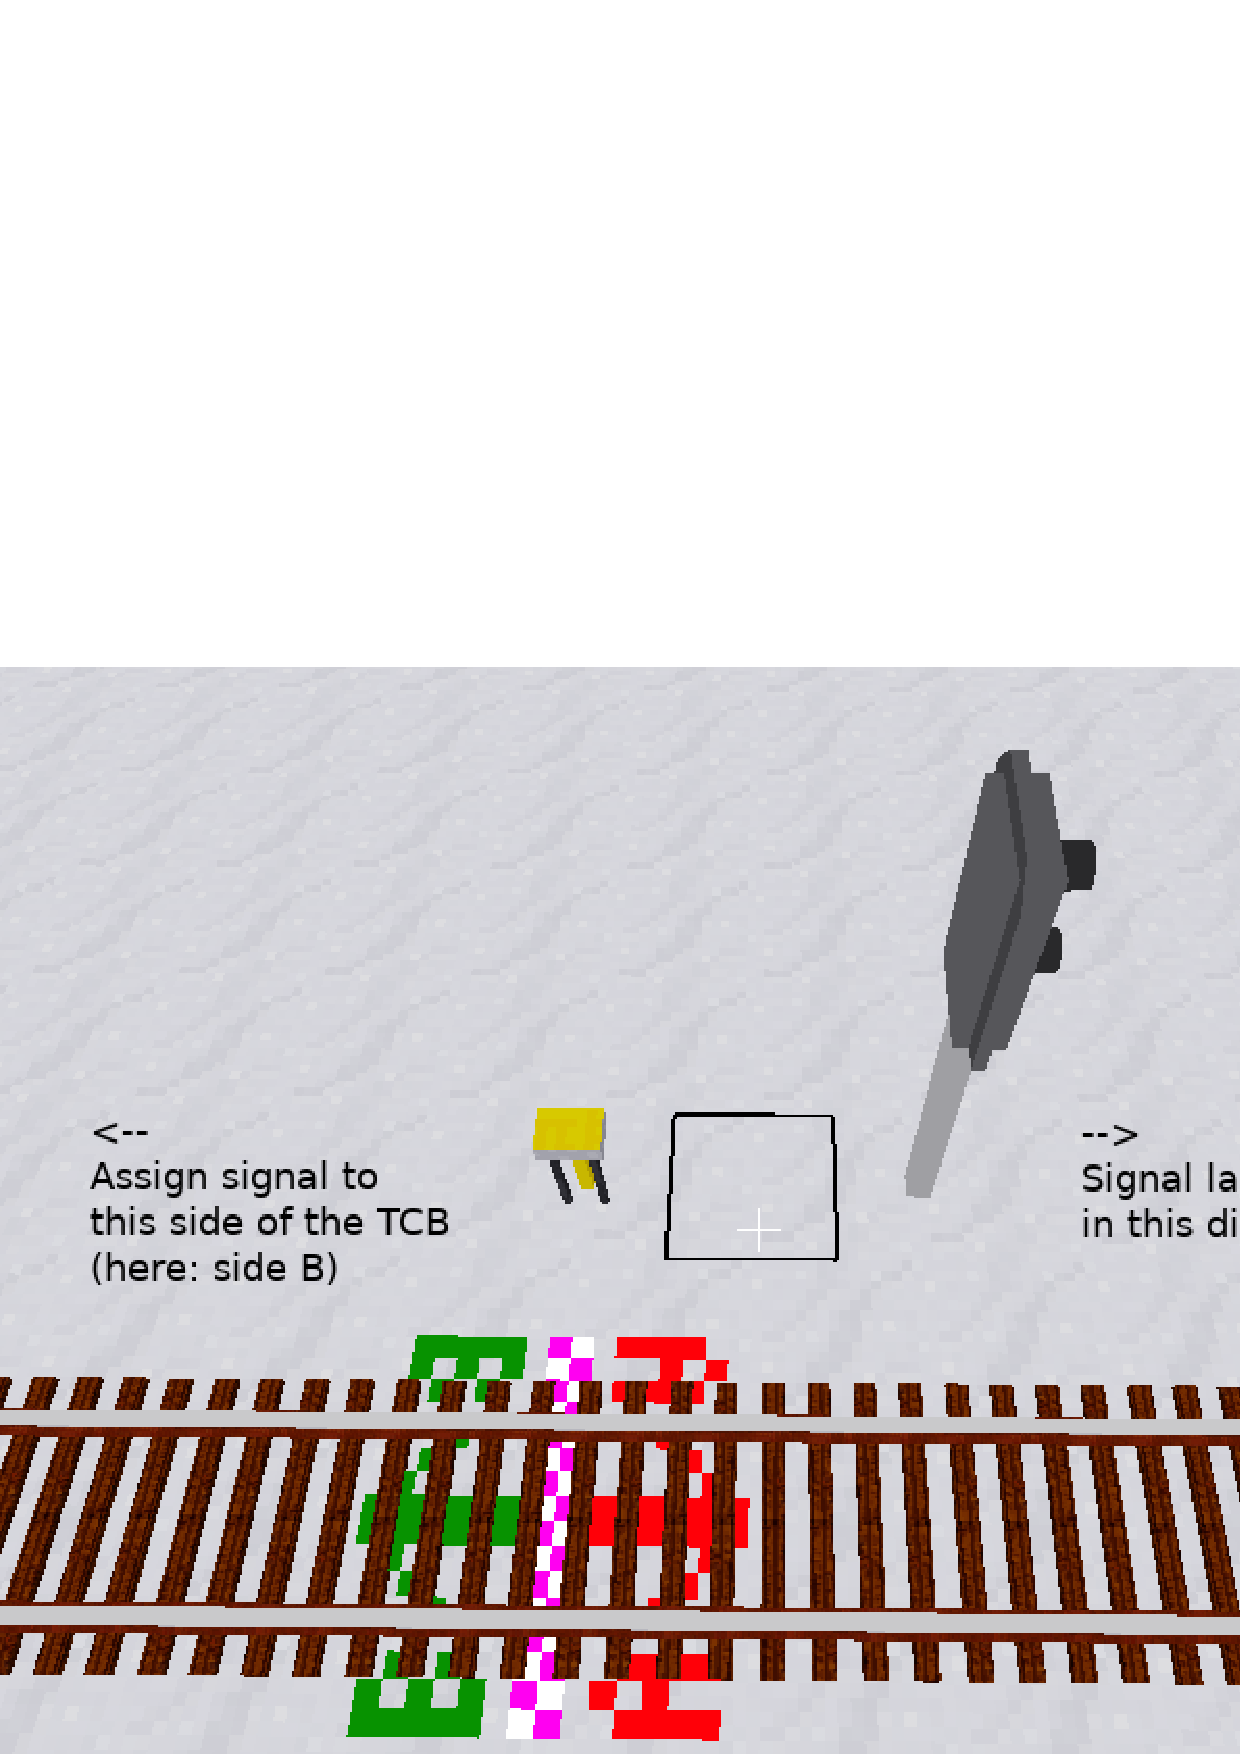
\includegraphics[width=8cm]{8_home_moritz_Home_Projekte_Minetest_minetest_mods_advtrains_assets_lyx_img_assign_signal.png}

If you haven't set an influence point for the signal yet, the influence
point formspec automatically opens.

You can assign a signal to each side of a TCB. This is, for example,
useful when creating block sections on a bi-directional main running
line.

Only main signals can ever be assigned to TCBs, because static ones
can either not display ``Danger'' or do not permit to proceed at
all.

\subsection{Shunt routes}

\textbf{The information in this section is subject to future change
because of safety issues!}

Operating railways is not all about driving trains around. Coupling,
decoupling and moving single engines, wagons or groups of wagons across
a station, called shunting, also plays an important role.

Remember what we said about routes: There must be no rail vehicles
on the route. So what if you have some goods wagons ready on a siding,
and want to couple an engine to it? You can not set a regular route
into the siding, because it is occupied.

The solution is to program a second route into the siding, but with
the difference that it already ends at the rear-facing signal of it,
so it doesn't include the siding section itself:

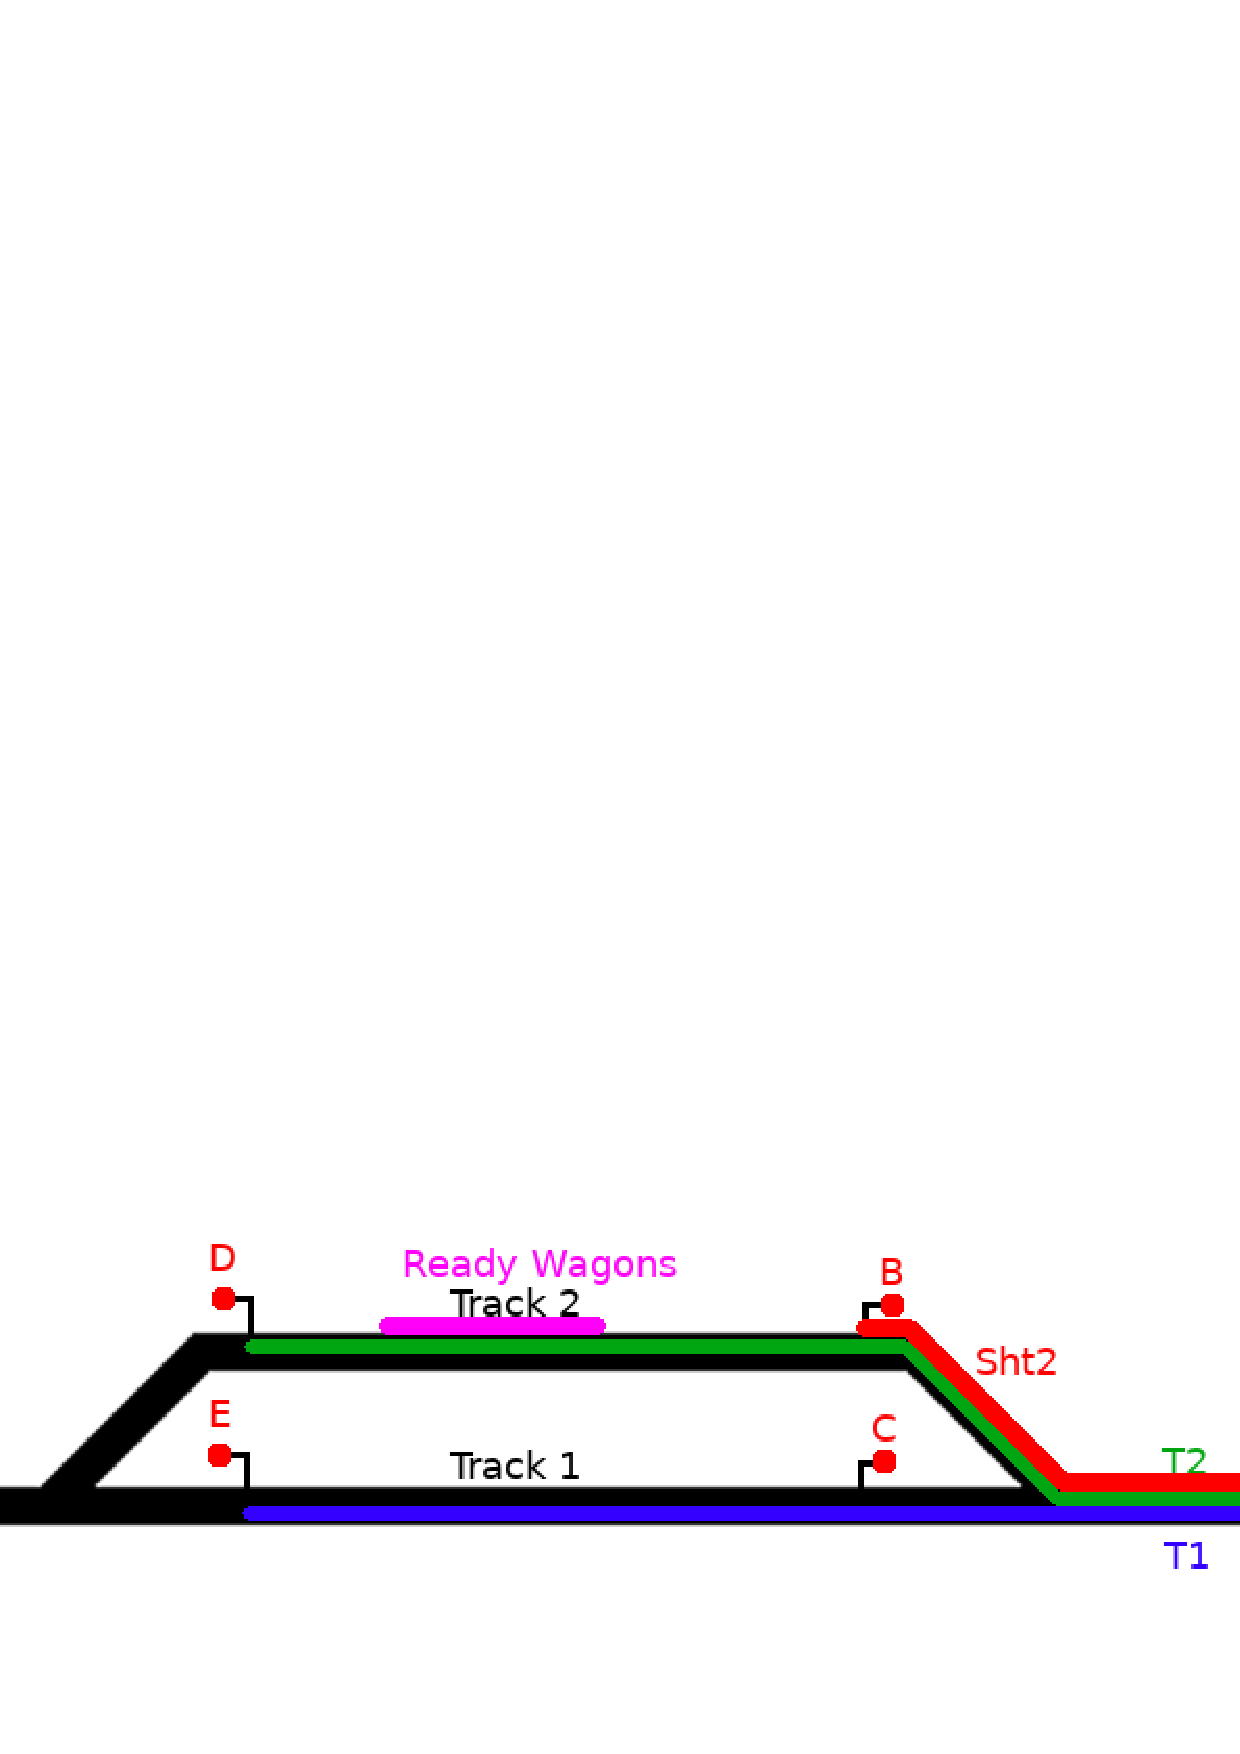
\includegraphics[width=7cm]{9_home_moritz_Home_Projekte_Minetest_minetest_mods_advtrains_assets_lyx_img_route_ex3.png}

The Sht2 route then needs to show a shunt aspect, which instructs
the driver to proceed slowly and watch out for vehicles on the route.
To show a ``free'' aspect here would be wrong, because that would
mean that the track is free until the next main signal, which it is
clearly not.

\textit{Note that advtrains\_interlocking currently does not allow
to set individual aspects for routes, this is a feature still to be
implemented soon.}

Shunt routes like this are, so far, the only exception to the ``Routes
should end at a signal facing the same direction'' rule.

\subsection{Route Release}

In early real-life interlocking systems, routes either had to be cancelled
by the signalman after the train had passed the route, or there was
a single release contact at the end of the route. However, as interlocking
systems evolved and the position of trains is now roughly known by
the track sections, portions of the route can be freed as soon as
the train has left the corresponding section.

AdvTrains has chosen a modern approach to route releasing. Each turnout
lock is associated to a track section belonging to the route's path.
Once the train leaves this section, all assigned locks are also freed.

Please note that reversing a train outside of stations is not only
discouraged, but also very dangerous, because even real-world interlocking
system do not expect this. There is a clear, human-sense rule that
you should never reverse the driving direction of a train while on
a main line or on a turnout. Else, you can be considered a terrorist.
(quote from professional!)

\subsection{Programming a route}

The route programming procedure is quite straightforward if you've
read the previous sections and understood how routes should be set.

Routes always start at a main signal. You must have assigned the signal
to a TCB, as described earlier.

When you right-click the main signal, it no longer changes its aspect.
Instead, a formspec pops up, showing you an (empty) list of routes
with the possibility to set them or to create new routes. Click the
``Create new route'' button to start programming a new route.

The form closes, and an arrow is displayed on the TCB. You are now
in ``Route Programming'' mode, programming the first track section
of the route. Now:
\begin{itemize}
\item Put any turnouts you need to lock in the correct position (e.g. by
right-clicking them). This includes flank protection.
\item Punch them. This makes a marker with a blue lock symbol appear.
\item If you punch a turnout again, or punch the marker, you can remove
the lock again.
\item When you've locked all turnouts in the current section, go to and
punch the TCB that is the border to the next track section the train
proceeds into.
\end{itemize}
Depending on the situation, you are now offered some possibilities
to proceed:
\begin{itemize}
\item Click the ``Advance to next section'' button if your route consists
of more sections with turnouts to lock, and you need to continue programming.
Follow the above steps to set locks for the next section.
\end{itemize}
Once you've clicked the ``Advance'' button, the lock markers change
to a red lock symbol, telling they can't be changed anymore. Repeat
the above procedure until you are ready to complete the programming
procedure:
\begin{itemize}
\item Click the ``Finish route HERE'' button when you've set up the locks
for the last track section of the route and punched the final TCB
(the one with the next signal). You will be asked for a route name
and your route will be saved.
\item The ``Finish route at end of NEXT section'' button (third button)
is an useful quickhand to make the route proceed one more section.
Using this button is equivalent to first clicking the ``Advance''
button, then flying to the end of the next track section and finishing
the route there. You can not (officially) set turnout locks in the
final section using this method.
\end{itemize}
A few hints:
\begin{itemize}
\item If one turnout should be locked by more than one section, set the
lock only in the \texttt{\textbf{last}} of those sections. Locking
the same turnout in multiple sections of a single route results in
undefined behavior!
\item If you accidentally advanced the route wrongly, you can use the ``Step
back one section'' button to undo this.
\item If you want to stop programming the entire route without saving it,
use the ``Cancel route programming'' button.
\item The third button is especially useful for programming simple block
sections on a main running line, since you can stay at the starting
signal (punch starting TCB and select third button).
\item If a route should end in a dead end, you MUST use the ``Finish in
NEXT section'' button, because there is no final TCB that you could
punch.
\item The third button does NOT work on sections with more than 2 exits,
because the system won't be able to determine the final TCB of the
route then.
\end{itemize}

\section{Interlocking system operation}

Setting up the interlocking for a portion of a railway network requires
some time, experience and planning, but once done, there's not much
to do anymore to make trains run on your, now safer, railway. This
section covers some useful practices to route trains across your network.

At the moment, routes can either be set by clicking the signal or
via LuaATC, or by using the ``Remote Routesetting'' button from
the Onboard Computer. It is planned to control this via a ``signal
box'' view based on the currently broken itrainmap.

\subsection{Train Safety System}

The Train Safety System, called ``LZB'' in the code (from the german
term Linienzugbeeinflussung, although this is a completely different
system), ensures that trains obey any restrictions imposed by signals
when influence points are set. This way, it is not possible to pass
signals at danger or to bypass speed restrictions.

It is possible to overrun red signals, if a route is cancelled while
a train is approaching. Real interlocking systems use a mechanism
called Approach locking for this, however, as of now, there's no similar
system in this mod. If a red signal is overrun, the train brakes using
emergency brake (``BB'') and can not be moved any further. You should
then examine the situation and drive the train backwards out of the
section.

As of now, changing the driving direction of a train always clears
any imposed speed restrictions.

\subsection{Simple route setting and cancelling}

To set a route, simply right-click the signal, select a route and
click ``set route''. If there are no conflicts, the signal turns
green and the train is allowed to proceed.

It may be possible that the route can not be set, because one or more
other routes conflict with the current one, or a section is blocked.
In this case, the signal stays red, and the conflicting item is shown
in the formspec. As soon as the conflict is resolved (by cancellation
or release of the conflicting route, or the section becoming free),
the requested route will be set and the signal turns green.

If a route is either requested or set, it can be cancelled from the
signalling formspec. This means that all turnouts and sections are
released, and the signal reverts back to red. This of course only
works when the train has not passed the signal yet. There is no mechanism
for Approach Locking.

\subsection{Automatic Working}

Block signals on main running lines usually only have a single route
to set, the one proceeding along the main line. Their purpose is only
to show whether there are trains in the next section. So, it would
be convenient if this only route would set itself again after a train
passed.

This is what Automatic Working is for. Set a route, click ``Enable
Automatic Working'', and as soon as a train passes, the route is
automatically re-set.

This function is nearly identical to SimSig automatic signals. It
can also be useful on a line with high traffic, when there's a low-frequented
access to a siding. You'd enable automatic working for the main route
and cancel it only when you need a train to go into the siding.

\section{Final notes}

The interlocking system is mainly finished, though there are still
some plans and ideas. They include:
\begin{itemize}
\item Signalbox panels, as revival of itrainmap
\item Individual signal aspects for routes
\item Distant signals
\item On-Train head-up display for oncoming signals (they have something
like this in Czech Republic, I forgot how it's called.)
\end{itemize}
Apart from this, there's the large oncoming project of a new timetable-based
train automation system, but this will take some time to evolve and
is out of the scope of this document.

If you have any suggestions, corrections, improvements, criticism
or cute kittens and stuff, you can always contact me by various means
(Forum PM, E-Mail (orwell@bleipb.de), Linuxworks server chat a.s.o.).
Have fun!

- orwell
\end{document}
